
%%%%%%%%%%%%%%%%%%%%%%%%%%%%%%%%%%%%%%%%%%%%%%%%%%%%%%%%%%%%%%%%%%%%%%%%%%%%%%%%%%%%%%%%%%%%%%%%%%%%%%%%%%%%%%
% Article:
% Bootstrap Inference for the Area Under the ROC Curve
% Statistical Theory
%%%%%%%%%%%%%%%%%%%%%%%%%%%%%%%%%%%%%%%%%%%%%%%%%%%%%%%%%%%%%%%%%%%%%%%%%%%%%%%%%%%%%%%%%%%%%%%%%%%%%%%%%%%%%%%



\section{Background}
% \subsection{The ROC Curve}
\textbf{The ROC Curve}

The ROC curve characterizes the relationship between variables in a classification model. 
One one side is the categorical outcome, which in this paper is a binary indicator variable. 
The outcomes are referred to as positive or negative, according to whether the event occurs or does not. 
The other component is a classification variable. 
It is, ideally, monotonically related to the probability that the binary event will occur. 
The classification variable can be interpreted as a model prediction, which, for example, could include a credit score for the prediction of default. 
In practice, it is often the output of a classification model, which could range from standard models as logistic regression, to a variety nonparametric classification algorithms and machine learning methods.

The ROC curve is a parametric curve, plotting the true positive rate against the false positive rate. 
The curve is parameterized by the discrimination threshold, the value of the classification variable, above which observations are classified as positive. 
A particular point on this curve shows the classification error for observations observations correctly classified as positive, against those that are classified as positive but are truly negative.

The result can be used as a measurement of the frequency of correct interpretation of a signal for predicting a binary element of a message. 
In fact, the use of this curve for a measure of signal quality dates back to the days of assessing the quality of radio transmissions for military use.
Early references include \citet{peterson1954}, \citet{vanmeter1954} and \citet{wald1949} for uses in this context.
A later review can be found in \citet{hanley1989}, in which the statistic is used to assess the quality of medical diagnoses.
Recently, this curve has been used by the business community to assess the discriminatory power of variables used in classification models for predictive modeling.

Figure \ref{fig:ROCcurve1} shows an example of the Receiver Operating Characteristic Curve. 
It plots the True Positive Rate (TPR) on the vertical axis against the False Positive Rate (FPR) on the horizontal axis. 
These proportions are calculated for a particular value of the classification threshold, which the user can vary to make a classification more selective or more inclusive. 
The observations with classification variable above the classification threshold are classified as positive and the rates are then calculated according to whether that classification is correct in each case. 
In the bottom left corner, only the strongest signals are used to identify positive outcomes and, for an effective model, the ratio of correct to incorrect positive identifications should be greater than equal, implying a steeper slope. 
As the threshold is increased, progressively weaker signals are used to identify positive outcomes and the performance should decline, resulting in a declining slope. 
At the other extreme, the classification threshold will include nearly the entire sample, for which the accuracy will have declined enough to coincide with the sample-wide event rate. 


%%%%%%%%%%%%%%%%%%%%%%%%%%%%%%%%%%%%%%%%%%%%%%%%%%%%%%%%%%%%%%%%%%%%%%%%%%%%%%%%%%%%%%%%%%%%%%%%%%%%%%%%%%%%%%%


\begin{figure}[h!]

\begin{center}

    \caption{Receiver Operating Characteristic Curve} \label{fig:ROCcurve1}

        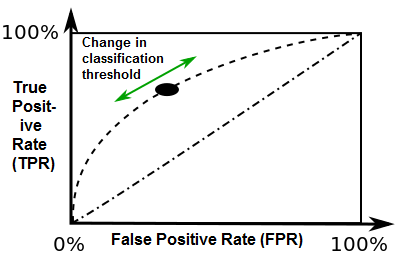
\includegraphics[scale=  0.75]{Figs/ROC/ROC_curve_3.png}



\end{center}

    \footnotesize

        \textbf{Receiver Operating Characteristic Curve:}
        True Positive Rate vs. False Positive Rate, for a particular value of the classification threshold. 
        Observations with classification variables above the classification threshold are classified as positive. 
        The true positive rate is the proportion of positive values of the classification that are correctly classified as negative, i.e. that lie above the threshold. 
        Conversely, the true negative rate is the proportion of negative values of the classification that are incorrectly classified as positive, also above the threshold. 
        The ROC curve is the parametric curve that is followed as the classification threshold varies from the highest to the lowest values in the sample. 

% Terms in $KLD(\textcolor{blue}{f_1}, \textcolor{red}{f_2})
%  = \sum_{k = 1}^{K} \left\{ \textcolor{magenta}{\big( f_1(t_k) - f_2(t_k) \big)}
%         \textcolor{orange}{\log \left( \frac{f_1(t_k)}{f_2(t_k)} \right)} \right\}$

\end{figure}


%%%%%%%%%%%%%%%%%%%%%%%%%%%%%%%%%%%%%%%%%%%%%%%%%%%%%%%%%%%%%%%%%%%%%%%%%%%%%%%%%%%%%%%%%%%%%%%%%%%%%%%%%%%%%%%



The better the model, the steeper will be the initial slope and the closer the curve will be to the upper boundaries. 
The area under this curve is the statistic that indicates the performance value of the classification variable. 
The diagonal line indicates the classifications that are no better than random allocation to positives and negatives. 
In this locus, the event rate is simply the average event rate for the entire sample. 
A model with a curve below this line is not effective in classifying, unless used in reverse order, when the curve will lie within the upper triangular region. 

\subsection{Area Under the ROC Curve}

The area under this curve can be computed directly by integration: 
% 
\begin{equation}
    A = \int_{-\infty}^{\infty} TPR(t) [-FPR^{\prime}(t)] dt, 
\end{equation}
% 
\noindent in which the true and false positive rates are defined as 
% 
\begin{equation}
    TPR(t) = \int_{t}^{\infty} f_y(t) dt \quad FPR(t) = \int_{t}^{\infty} f_x(t) dt. 
\end{equation}
% 
The distribution of the classification variable corresponding to positive outcomes is denoted by $y$ and that for negative outcomes is denoted by $x$. The functions $f_y(\cdot)$ and $f_x(\cdot)$ are the corresponding density functions. 
% 
A brief series of calculations will reveal this to be equivalent to the following probability
% 
\begin{equation}
    A = Prob{\left\{ y > x \right\}}.
\end{equation}
% 
This can be interpreted as an evaluation of a pairwise comparison of the correct ordering of predictions for all pairs of predictions that could be made in the sample. 
% 
Specifically, if one were to pick a pair of predictions, drawn randomly from predictions corresponding to pairs of the positive ($y$) and the negative ($x$) outcomes, the AUROC is the probability that these predictions are correctly ordered.
% 
The sample analogue is calculated as follows
%
\begin{equation} \label{eqn:auroc}
    \hat{A} = \hat{\Pr} \{ y > x \} = \frac{1}{m n} \sum_{i = 1}^{m} \sum_{j = 1}^{n} I_{\left\{ y_j > x_i \right\}}.
\end{equation}
% 



%\begin{equation}
%    \hat{A} = Prob{\left\{ y > x \right\}}
%\end{equation}
%
%\begin{equation}
%    \hat{A} = \frac{1}{m n} \sum_{i = 1}^{m} \sum_{j = 1}^{n} I_{\left\{ y_j > x_i \right\}}
%\end{equation}
%
%
%Definition of AUROC
%\begin{itemize}
%    \item Direct definition: Calculation of area by integration
%    \begin{itemize}
%        \item $\int_{-\infty}^{\infty} TPR(t) [-FPR^{\prime}(t)] dt $
%    \end{itemize}
%    \item Direct definition: Pairwise comparison of correct ordering of predictions for all pairs of predictions % from positive and negative outcomes
%    \begin{itemize}
%        \item $\hat{A} = \hat{\Pr} \{ y > x \} = \frac{1}{m n} \sum_{i = 1}^{m} \sum_{j = 1}^{n} I_{\left\{ y_j > x_i \right\}}$
%    \end{itemize}
%    \item In words: If you were to pick a pair of predictions, drawn randomly from predictions corresponding to pairs of the positive ($y$) and negative ($x$) outcomes, the AUROC is the probability that these predictions are correctly ordered.
%\end{itemize}




\textbf{Calculation}

This calculation is provided in \citet{hanleymcneil1982}, while an implementation of the calculation is made available in \citet{proc2011}.
This is an implementation of the approach taken in \citet{delong1988}. 
% 
A more efficient method of computation is proposed by \citet{sunxu2014}, which is a faster approach to calculating the quantities in \citet{hanleymcneil1982} (check reference), as well as those for \citet{delong1988}.
% 

\subsection{Volume interpretation}

Volume Under the Joint distribution of Predictor Variables

A more intuitive approach to the calculation of the AUROC is to visualize it as the probability mass that satisfies a certain condition. 
Consider the following joint distribution formed by the two groups of classification variables. 
Combine the marginal distributions of the classification variables corresponding to the positive and negative outcomes by simply multiplying the marginal distributions. 
The resulting joint density will represent the probability density of all possible pairs of $(x,y)$ pairs from the sample. 
Now restrict this space to the region defined by the indicator in \ref{eqn:auroc}, which is the region above the $y = x$ line. 
The area under the receiver operating curve is the volume under this ``receiver operating surface''. 

% This binormal approach is discussed next. 

% 

%%%%%%%%%%%%%%%%%%%%%%%%%%%%%%%%%%%%%%%%%%%%%%%%%%%%%%%%%%%%%%%%%%%%%%%%%%%%%%%%%%%%%%%%%%%%%%%%%%%%

\begin{figure}[h!]

\begin{center}

    \caption{AUROC Under the Binormal Classification Model} \label{fig:binorm1}

    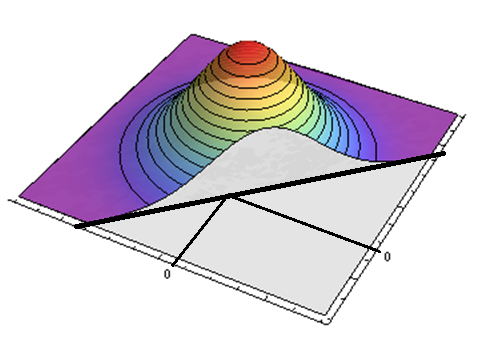
\includegraphics[scale=  0.500000]{Figs/Binormal/BivariateNormal1.png}

\end{center}

\footnotesize

    \textbf{AUROC Under the Binormal Classification Model:}

    Description goes here.

\end{figure}



%%%%%%%%%%%%%%%%%%%%%%%%%%%%%%%%%%%%%%%%%%%%%%%%%%%%%%%%%%%%%%%%%%%%%%%%%%%%%%%%%%%%%%%%%%%%%%%%%%%%




%%%%%%%%%%%%%%%%%%%%%%%%%%%%%%%%%%%%%%%%%%%%%%%%%%%%%%%%%%%%%%%%%%%%%%%%%%%%%%%%%%%%%%%%%%%%%%%%%%%%

\begin{figure}[h!]

\begin{center}

    \caption{Volume Under the ``ROC Surface''} \label{fig:volume1}

    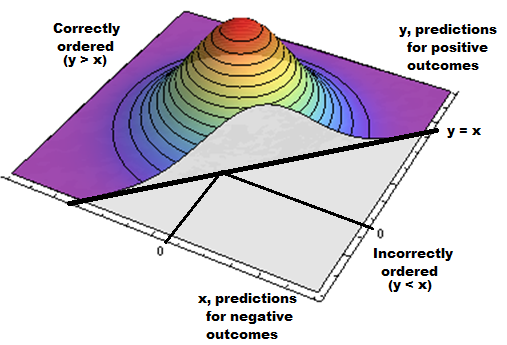
\includegraphics[scale=  0.500000]{Figs/Volume/AUROC_vol_3.png}

\end{center}

\footnotesize

    \textbf{Volume Under the ``ROC Surface'':}
    With the AUROC defined in the form $A = Prob{\left\{ y > x \right\}}$, it is clear that it can be visualized as the volume of the probability mass under the surface of the joint distribution of classification variables from positive and negative outcomes.

\end{figure}



%%%%%%%%%%%%%%%%%%%%%%%%%%%%%%%%%%%%%%%%%%%%%%%%%%%%%%%%%%%%%%%%%%%%%%%%%%%%%%%%%%%%%%%%%%%%%%%%%%%%





\subsection{Examples}

\textbf{Binormal Model}

The above example illustrates the calculation of the AUROC for the specific case of the binormal model. 
The calculation is known to be equivalent to the normal CDF evaluated at the value of a test statistic for the difference between the two normal distributions. 
Similarly, the variability of the estimate results in confidence bounds that are also calculated by the normal CDF, which is specified in \citet{demidenko2012}. 
However, it is noteworthy that the fact that the statistic is a function of the test statistic for a test of the difference between the pair of distributions of classification variables. 
% 

\textbf{Biexponential Model}

Another possibility is the biexponential model, in which both sets of classification variables are drawn from exponential distributions. 
% 
This alternative is featured in \citet{hanleymcneil1982} for a calculation of the variance of the AUROC.
This approach allows for a more generic formulation that is calculated directly from the empirical distributions of the classification variables from both the positive and negative outcomes.
% 

Features of these two examples can be extended to the study of generic models for classification. 
However, parametric solutions are not preferred in the literature, since the classification model is likely to be much more unstructured than a parametric model would allow.
A nonparametric solution is not only possible but preferred by users in industry. 
Regardless of the particular model, the parametric examples can still be used to explain an important correspondence between modeling methods. 
The mapping presented next is generalized to all classification models. 

\subsection{An important correspondence}

% Predicting Outcomes vs. Measuring Difference

There is an important similarity between the activity of creating a classification model and of comparing two distributions. 
% 
A difference of the distributions is a necessary condition for a classification variable to have predictive power for the binary outcome. 
Conversely, if the classification variable produces predictions with an AUROC above $0.5$, then the distributions must be different. 
% 
For this reason, an important connection can be made between nonparametric statistics and the AUROC, and this connection is useful for finding ways to further characterize the AUROC. 

% 
%%%%%%%%%%%%%%%%%%%%%%%%%%%%%%%%%%%%%%%%%%%%%%%%%%%%%%%%%%%%%%%%%%%%%%%%%%%%%%%%%%%%%%%%%%%%%%%%%%%%%%%%%%%%%%%



\begin{figure}[h!]

\begin{center}

    \caption{Equivalence of Classification Models} \label{fig:classification1}

    \begin{tabular}{c}

        \subfloat[Classification Model]{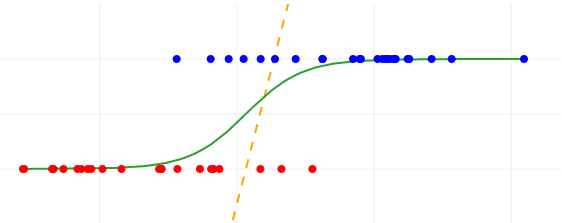
\includegraphics[scale=  0.50]{Figs/Classification/LogisticReg2.png}} \\


        \subfloat[Difference of Distributions]{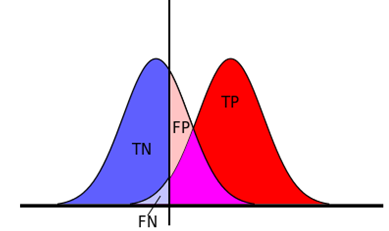
\includegraphics[scale=  0.50]{Figs/Classification/ClassModelDistns1.png}} \\




    \end{tabular}

\end{center}

    \footnotesize
    
        \textbf{Equivalence of Classification Models: }
        Description goes here.
        
\end{figure}


%%%%%%%%%%%%%%%%%%%%%%%%%%%%%%%%%%%%%%%%%%%%%%%%%%%%%%%%%%%%%%%%%%%%%%%%%%%%%%%%%%%%%%%%%%%%%%%%%%%%%%%%%%%%%%%



%%%%%%%%%%%%%%%%%%%%%%%%%%%%%%%%%%%%%%%%%%%%%%%%%%%%%%%%%%%%%%%%%%%%%%%%%%%%%%%%%%%%%%%%%%%%%%%%%%%%%%%%%%%%%%%


\begin{figure}
        \begin{minipage}[b]{0.45\linewidth}
            \centering
            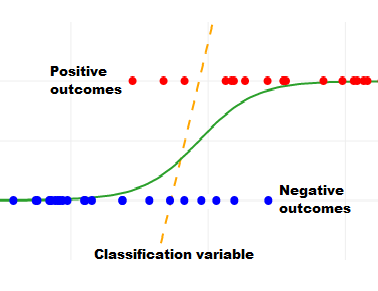
\includegraphics[width=\textwidth]{Figs/Classification/LogisticReg_5.png}
            % \caption{Predictive value of variables \\ (relation of score to positives and negatives)}
            \caption{Predictive value of classification variables}
        \end{minipage}
        \hspace{0.5cm}
        \begin{minipage}[b]{0.45\linewidth}
            \centering
            \includegraphics[width=\textwidth]{Figs/Classification/ROC_distns_1.png}
            % \caption{Difference in distributions of variables \\ (positives vs. negatives)}
            \caption{Difference in the distributions of variables}
        \end{minipage}
    % 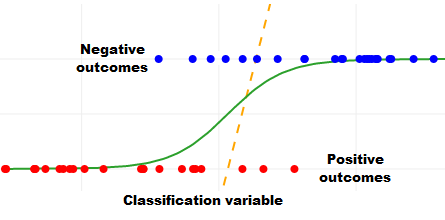
\includegraphics[scale =  0.5 ]{Figs/LogisticReg_3.png}%
    % \includegraphics[scale =  0.5 ]{Figs/ROC_distns_1.png}
\end{figure}




%\begin{figure}[h!]
%
%\begin{center}
%
%    \caption{Equivalence of Classification Models} \label{fig:classification1}
%
%    \begin{tabular}{c}
%
%        \subfloat[Classification Model]{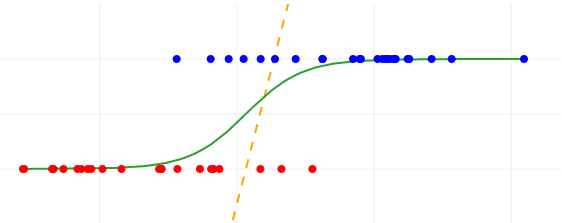
\includegraphics[scale=  0.50]{Figs/Classification/LogisticReg2.png}} \\
%
%
%        \subfloat[Difference of Distributions]{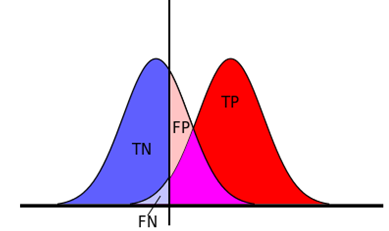
\includegraphics[scale=  0.50]{Figs/Classification/ClassModelDistns1.png}} \\
%
%
%
%
%    \end{tabular}
%
%\end{center}
%
%    \footnotesize
%
%        \textbf{Equivalence of Classification Models: }
%        Description goes here.
%
%\end{figure}


%%%%%%%%%%%%%%%%%%%%%%%%%%%%%%%%%%%%%%%%%%%%%%%%%%%%%%%%%%%%%%%%%%%%%%%%%%%%%%%%%%%%%%%%%%%%%%%%%%%%%%%%%%%%%%%






\subsection{Equivalence to Ranking Statistics}

Because of this close connection between statistical methodologies, a number of methods in the nonparametric literature are useful for analyzing the AUROC. 
Nonparametric ranking statistics are described in \citet{lehmann2006} and \citet{kendall1990}, in reference to the literature on comparison of distributions. .
One method that stands out as especially relevant is the 
Mann-Whitney $U$-statistic, which is presented in \citet{mannwhitney1947}. 
% 
\begin{equation}
    U = \sum_{i = 1}^{m} \sum_{j = 1}^{n} I_{\left\{ y_j > x_i \right\}}
\end{equation}
% 
This is the same as AUROC, without the normalization by the count of pairs $m n$.

This equivalence is leveraged for computational advantage, since the $U$-statistic is calculated as follows.
First, sort the observations in increasing order.
Then, assign ranks to the observations, with $1$ for the smallest score and the sample size for the observation with the largest score.
Finally, take the sum of the ranks corresponding to the positive outcomes and subtract the following quantity.
\begin{equation}
    \frac{1}{2} n_1(n_1 + 1)
\end{equation}
% 
A similar statistic is \citet{wilcoxon1945} for similar purposes.
All of these 
It was in 
\citet{bamber1975} that the connection was made between the AUROC and the Mann-Whitney $U$-statistic.
Other approaches for evaluating classification models are similarly inspired by tools such as
Somers' $d$ (\citet{somers1962}) and Kendall's $\tau$ (see \citet{kendall1990})
A simulation-based approach to modeling the variability of these statistics is found in \citet{newson2006}, which involved jackknifing the numerator and denominator of the ratio in Kendall's $\tau$ and taking a Taylor expansion. 

The connection to the ranking statistics in the nonparametric literature is appealing to practitioners, since it precludes the need for parametric modeling of distributions that may be highly unstructured. 
While the ranking statistics above are intended to compare differences in sampling distributions, the mathematical equivalence to the classification problem opens up the possibility of using these approaches to evaluate models, without imposing parametric restrictions. 


\textbf{Why this approach}
Taken together, with the equivalence of the ranking problem to the classification problem, 
% 
one can conclude that the variation of distributions of scores is of paramount importance. 
This is especially so, since the AUROC statistic is the sum of the volume under the joint distribution defined by the classification distributions themselves. 
Any variation in these distributions can cause material variation in the value of the AUROC. 


\subsection{A ``Non-parametric'' Solution}

Taken together, these ranking statistics highlight the fact that the AUROC is inherently nonparametric measure of performance. 
It is often used in combination with modeling techniques that are also nonparametric. 
% 
In some circles in industry, there is a general distaste for parametric assumptions, particularly when not supported by the data, especially in when there is access to large datasets, that can reveal the structure of the data with more precision. 
% 
In this context, there is little justification for imposing a parametric specification for variation in distributions, when parametric distributions are not used for the distributions themselves. 
% 
In particular, the change in classification distributions can be summarized by a nonparametric distance measurement and what follows is a discussion of the relevance of such a distance. 

%\begin{itemize}
%    \item AUROC is inherently nonparametric measure of performance
%    \begin{itemize}
%        \item General distaste for parametric assumptions, particularly when not supported by the data
%        \item Little justification to impose parametric specification for variation in distributions, when parametric distributions are not used for the distributions themselves
%    \end{itemize}
%    \item Change in distribution is summarized by a distance measurement
%    \item Prediction interval: The set of all possible distributions this distance from the distributions in the sample
%\end{itemize}



\textbf{Distance}

In practice, a business user would track the performance of a model while it is in use for making business decisions. 
If the model is run continuously, it is prudent to take periodic measurements in AUROC. 
It is also worth monitoring the variability in distributions of classification variables passing through the model. 
Once any model moves into uncharted territory, there arises the possibility that the predictions are no longer valid, in the case that the functional form cannot be extrapolated beyond the support of the build sample. 
It would not be a problem, so long as the specification were correct throughout the domain of the model. 
However, in the classification problem, the distributions themselves are of first order importance, since this defines the measurement of the statistic itself. 
A careful use of a classification model would involve a specification of the terms under which the model will be discontinued or scheduled for rebuild with new data. 
If it is the case that the model is planned to be used for situations in which the variables have distributions sufficiently similar to the original build distribution, then the AUROC statistic can be expected to vary accordingly, over the foreseeable lifespan of the model. 
It is for this reason that the prediction intervals are proposed that take into account this variation. 
% 
%\begin{itemize}
%    \item In practice, track performance of model while in use
%    \begin{itemize}
%        \item take AUROC measurements periodically
%    \end{itemize}
%    \item Also, track evolution of distributions of predictions
%    \begin{itemize}
%        \item take periodic measurements of changes in distributions from build sample
%    \end{itemize}
%    \item Extreme changes in either would trigger rebuild of the model
%    \item Prediction intervals should allow for this level of variability
%\end{itemize}
% 
In order to quantify this variation, a distance measure is required for the calculation of the bounds of these intervals. 
% As the modeling techniques and the evaluation methods are typically nonparametric, it is worthwhile to maintain a nonparametric measure of distance as well.
%
% Define $D()$ but no more, until after optimization problem. 
% Next, optimization problem. 
%
This will be presented in the following section, after the formal specification of the modeling problem. 



%%%%%%%%%%%%%%%%%%%%%%%%%%%%%%%%%%%%%%%%%%%%%%%%%%%%%%%%%%%%%%%%%%%%%%%%%%%%%%%%%%%%%%%%%%%%%%%%%%%%%%%%%%%%%%%
%%%%%%%%%%%%%%%%%%%%%%%%%%%%%%%%%%%%%%%%%%%%%%%%%%%%%%%%%%%%%%%%%%%%%%%%%%%%%%%%%%%%%%%%%%%%%%%%%%%%%%%%%%%%%%%
